\documentclass[]{article}
\usepackage{lmodern}
\usepackage{amssymb,amsmath}
\usepackage{ifxetex,ifluatex}
\usepackage{fixltx2e} % provides \textsubscript
\ifnum 0\ifxetex 1\fi\ifluatex 1\fi=0 % if pdftex
  \usepackage[T1]{fontenc}
  \usepackage[utf8]{inputenc}
\else % if luatex or xelatex
  \ifxetex
    \usepackage{mathspec}
  \else
    \usepackage{fontspec}
  \fi
  \defaultfontfeatures{Ligatures=TeX,Scale=MatchLowercase}
\fi
% use upquote if available, for straight quotes in verbatim environments
\IfFileExists{upquote.sty}{\usepackage{upquote}}{}
% use microtype if available
\IfFileExists{microtype.sty}{%
\usepackage{microtype}
\UseMicrotypeSet[protrusion]{basicmath} % disable protrusion for tt fonts
}{}
\usepackage[margin=1in]{geometry}
\usepackage{hyperref}
\hypersetup{unicode=true,
            pdftitle={02\_Differential\_analysis},
            pdfauthor={Aurelien Dugourd},
            pdfborder={0 0 0},
            breaklinks=true}
\urlstyle{same}  % don't use monospace font for urls
\usepackage{color}
\usepackage{fancyvrb}
\newcommand{\VerbBar}{|}
\newcommand{\VERB}{\Verb[commandchars=\\\{\}]}
\DefineVerbatimEnvironment{Highlighting}{Verbatim}{commandchars=\\\{\}}
% Add ',fontsize=\small' for more characters per line
\usepackage{framed}
\definecolor{shadecolor}{RGB}{248,248,248}
\newenvironment{Shaded}{\begin{snugshade}}{\end{snugshade}}
\newcommand{\AlertTok}[1]{\textcolor[rgb]{0.94,0.16,0.16}{#1}}
\newcommand{\AnnotationTok}[1]{\textcolor[rgb]{0.56,0.35,0.01}{\textbf{\textit{#1}}}}
\newcommand{\AttributeTok}[1]{\textcolor[rgb]{0.77,0.63,0.00}{#1}}
\newcommand{\BaseNTok}[1]{\textcolor[rgb]{0.00,0.00,0.81}{#1}}
\newcommand{\BuiltInTok}[1]{#1}
\newcommand{\CharTok}[1]{\textcolor[rgb]{0.31,0.60,0.02}{#1}}
\newcommand{\CommentTok}[1]{\textcolor[rgb]{0.56,0.35,0.01}{\textit{#1}}}
\newcommand{\CommentVarTok}[1]{\textcolor[rgb]{0.56,0.35,0.01}{\textbf{\textit{#1}}}}
\newcommand{\ConstantTok}[1]{\textcolor[rgb]{0.00,0.00,0.00}{#1}}
\newcommand{\ControlFlowTok}[1]{\textcolor[rgb]{0.13,0.29,0.53}{\textbf{#1}}}
\newcommand{\DataTypeTok}[1]{\textcolor[rgb]{0.13,0.29,0.53}{#1}}
\newcommand{\DecValTok}[1]{\textcolor[rgb]{0.00,0.00,0.81}{#1}}
\newcommand{\DocumentationTok}[1]{\textcolor[rgb]{0.56,0.35,0.01}{\textbf{\textit{#1}}}}
\newcommand{\ErrorTok}[1]{\textcolor[rgb]{0.64,0.00,0.00}{\textbf{#1}}}
\newcommand{\ExtensionTok}[1]{#1}
\newcommand{\FloatTok}[1]{\textcolor[rgb]{0.00,0.00,0.81}{#1}}
\newcommand{\FunctionTok}[1]{\textcolor[rgb]{0.00,0.00,0.00}{#1}}
\newcommand{\ImportTok}[1]{#1}
\newcommand{\InformationTok}[1]{\textcolor[rgb]{0.56,0.35,0.01}{\textbf{\textit{#1}}}}
\newcommand{\KeywordTok}[1]{\textcolor[rgb]{0.13,0.29,0.53}{\textbf{#1}}}
\newcommand{\NormalTok}[1]{#1}
\newcommand{\OperatorTok}[1]{\textcolor[rgb]{0.81,0.36,0.00}{\textbf{#1}}}
\newcommand{\OtherTok}[1]{\textcolor[rgb]{0.56,0.35,0.01}{#1}}
\newcommand{\PreprocessorTok}[1]{\textcolor[rgb]{0.56,0.35,0.01}{\textit{#1}}}
\newcommand{\RegionMarkerTok}[1]{#1}
\newcommand{\SpecialCharTok}[1]{\textcolor[rgb]{0.00,0.00,0.00}{#1}}
\newcommand{\SpecialStringTok}[1]{\textcolor[rgb]{0.31,0.60,0.02}{#1}}
\newcommand{\StringTok}[1]{\textcolor[rgb]{0.31,0.60,0.02}{#1}}
\newcommand{\VariableTok}[1]{\textcolor[rgb]{0.00,0.00,0.00}{#1}}
\newcommand{\VerbatimStringTok}[1]{\textcolor[rgb]{0.31,0.60,0.02}{#1}}
\newcommand{\WarningTok}[1]{\textcolor[rgb]{0.56,0.35,0.01}{\textbf{\textit{#1}}}}
\usepackage{graphicx,grffile}
\makeatletter
\def\maxwidth{\ifdim\Gin@nat@width>\linewidth\linewidth\else\Gin@nat@width\fi}
\def\maxheight{\ifdim\Gin@nat@height>\textheight\textheight\else\Gin@nat@height\fi}
\makeatother
% Scale images if necessary, so that they will not overflow the page
% margins by default, and it is still possible to overwrite the defaults
% using explicit options in \includegraphics[width, height, ...]{}
\setkeys{Gin}{width=\maxwidth,height=\maxheight,keepaspectratio}
\IfFileExists{parskip.sty}{%
\usepackage{parskip}
}{% else
\setlength{\parindent}{0pt}
\setlength{\parskip}{6pt plus 2pt minus 1pt}
}
\setlength{\emergencystretch}{3em}  % prevent overfull lines
\providecommand{\tightlist}{%
  \setlength{\itemsep}{0pt}\setlength{\parskip}{0pt}}
\setcounter{secnumdepth}{0}
% Redefines (sub)paragraphs to behave more like sections
\ifx\paragraph\undefined\else
\let\oldparagraph\paragraph
\renewcommand{\paragraph}[1]{\oldparagraph{#1}\mbox{}}
\fi
\ifx\subparagraph\undefined\else
\let\oldsubparagraph\subparagraph
\renewcommand{\subparagraph}[1]{\oldsubparagraph{#1}\mbox{}}
\fi

%%% Use protect on footnotes to avoid problems with footnotes in titles
\let\rmarkdownfootnote\footnote%
\def\footnote{\protect\rmarkdownfootnote}

%%% Change title format to be more compact
\usepackage{titling}

% Create subtitle command for use in maketitle
\providecommand{\subtitle}[1]{
  \posttitle{
    \begin{center}\large#1\end{center}
    }
}

\setlength{\droptitle}{-2em}

  \title{02\_Differential\_analysis}
    \pretitle{\vspace{\droptitle}\centering\huge}
  \posttitle{\par}
    \author{Aurelien Dugourd}
    \preauthor{\centering\large\emph}
  \postauthor{\par}
      \predate{\centering\large\emph}
  \postdate{\par}
    \date{5/12/2020}


\begin{document}
\maketitle

\hypertarget{license-info}{%
\subsubsection{License Info}\label{license-info}}

This program is free software: you can redistribute it and/or modify it
under the terms of the GNU General Public License as published by the
Free Software Foundation, either version 3 of the License, or (at your
option) any later version.

This program is distributed in the hope that it will be useful, but
WITHOUT ANY WARRANTY; without even the implied warranty of
MERCHANTABILITY or FITNESS FOR A PARTICULAR PURPOSE. See the GNU General
Public License for more details.

Please check \url{http://www.gnu.org/licenses/}.

\hypertarget{introduction}{%
\subsection{Introduction}\label{introduction}}

Here we present examples of differential analysis of omic dataset, using
RNAseq for the present case.

\hypertarget{getting-started}{%
\subsection{Getting Started}\label{getting-started}}

We first load the required libraries.

\begin{Shaded}
\begin{Highlighting}[]
\CommentTok{#Main libraries}
\KeywordTok{library}\NormalTok{(readr)}
\KeywordTok{library}\NormalTok{(limma)}

\CommentTok{#Support functions also requires}
\KeywordTok{library}\NormalTok{(ggplot2)}
\KeywordTok{library}\NormalTok{(reshape)}
\KeywordTok{library}\NormalTok{(pheatmap)}
\KeywordTok{library}\NormalTok{(gridExtra)}
\KeywordTok{library}\NormalTok{(grid)}
\KeywordTok{library}\NormalTok{(cowplot)}
\KeywordTok{library}\NormalTok{(ggrepel)}
\KeywordTok{library}\NormalTok{(hexbin)}

\CommentTok{#Import the support funciton script }
\CommentTok{#/!\textbackslash{}/!\textbackslash{} PATH MAY NEED TO BE ADAPTED /!\textbackslash{}/!\textbackslash{}}
\CommentTok{#/!\textbackslash{}/!\textbackslash{} Don't forget to set working directory /!\textbackslash{}/!\textbackslash{}}

\KeywordTok{source}\NormalTok{(}\StringTok{"scripts/support_functions.R"}\NormalTok{)}
\end{Highlighting}
\end{Shaded}

\hypertarget{import-the-normalised-dataframe-and-experiemental-design}{%
\subsubsection{Import the normalised dataframe and experiemental
design}\label{import-the-normalised-dataframe-and-experiemental-design}}

\begin{Shaded}
\begin{Highlighting}[]
\CommentTok{#Data}
\NormalTok{count_df_vsn <-}\StringTok{ }\KeywordTok{as.data.frame}\NormalTok{(}\KeywordTok{read_csv}\NormalTok{(}\StringTok{"data/count_df_vsn.csv"}\NormalTok{))}
\end{Highlighting}
\end{Shaded}

\begin{verbatim}
## Parsed with column specification:
## cols(
##   gene = col_character(),
##   PANC1.WT.Rep1 = col_double(),
##   PANC1.WT.Rep2 = col_double(),
##   PANC1.WT.Rep3 = col_double(),
##   PANC1.FOXA2KO.Rep1 = col_double(),
##   PANC1.FOXA2KO.Rep2 = col_double(),
##   PANC1.FOXA2KO.Rep3 = col_double()
## )
\end{verbatim}

\begin{Shaded}
\begin{Highlighting}[]
\KeywordTok{row.names}\NormalTok{(count_df_vsn) <-}\StringTok{ }\NormalTok{count_df_vsn[,}\DecValTok{1}\NormalTok{]}
\NormalTok{count_df_vsn <-}\StringTok{ }\NormalTok{count_df_vsn[,}\OperatorTok{-}\DecValTok{1}\NormalTok{]}
\CommentTok{#Design}
\NormalTok{targets <-}\StringTok{ }\KeywordTok{as.data.frame}\NormalTok{(}\KeywordTok{read_csv}\NormalTok{(}\StringTok{"support/targets.csv"}\NormalTok{))}
\end{Highlighting}
\end{Shaded}

\begin{verbatim}
## Parsed with column specification:
## cols(
##   sample = col_character(),
##   condition = col_character()
## )
\end{verbatim}

\hypertarget{limma-differential-analysis}{%
\subsubsection{LIMMA differential
analysis}\label{limma-differential-analysis}}

now let's run a simple differential analysis using a simple wrapper for
such situation

\begin{Shaded}
\begin{Highlighting}[]
\CommentTok{#first check the conditions order}
\KeywordTok{unique}\NormalTok{(targets}\OperatorTok{$}\NormalTok{condition)}
\end{Highlighting}
\end{Shaded}

\begin{verbatim}
## [1] "PANC1.WT"      "PANC1.FOXA2KO"
\end{verbatim}

\begin{Shaded}
\begin{Highlighting}[]
\CommentTok{#we want to compare the KO with the WT so we build a comparison list}
\NormalTok{comparisons <-}\StringTok{ }\KeywordTok{list}\NormalTok{(}\StringTok{"KOvsWT"}\NormalTok{ =}\StringTok{ }\KeywordTok{c}\NormalTok{(}\DecValTok{2}\NormalTok{,}\OperatorTok{-}\DecValTok{1}\NormalTok{)) }\CommentTok{#each vector of the list represent the contrasts, here we substract the first condition (-1) to the second one (2)}

\CommentTok{#now that the comparisons are defined, we can run limma}
\NormalTok{limmaRes <-}\StringTok{ }\KeywordTok{runLimma}\NormalTok{(}\DataTypeTok{measurements =}\NormalTok{ count_df_vsn, }
                     \DataTypeTok{targets =}\NormalTok{ targets, }
                     \DataTypeTok{comparisons =}\NormalTok{ comparisons)}
\end{Highlighting}
\end{Shaded}

\begin{verbatim}
##               V1
## PANC1.WT      -1
## PANC1.FOXA2KO  1
\end{verbatim}

\begin{Shaded}
\begin{Highlighting}[]
\CommentTok{#once limma has run, we extract the statistic dataframe summarise the differential analysis}
\NormalTok{ttop_KOvsWT <-}\StringTok{ }\KeywordTok{ttopFormatter}\NormalTok{(}\KeywordTok{topTable}\NormalTok{(limmaRes[[}\DecValTok{1}\NormalTok{]], }\DataTypeTok{coef =} \DecValTok{1}\NormalTok{, }\DataTypeTok{number =} \KeywordTok{length}\NormalTok{(count_df_vsn[,}\DecValTok{1}\NormalTok{]), }\DataTypeTok{adjust.method =} \StringTok{"fdr"}\NormalTok{))}

\NormalTok{##make a qqplot}
\NormalTok{null_model <-}\StringTok{ }\KeywordTok{pnorm}\NormalTok{(}\KeywordTok{rnorm}\NormalTok{(}\KeywordTok{length}\NormalTok{(ttop_KOvsWT[,}\DecValTok{1}\NormalTok{])))}
\KeywordTok{plot}\NormalTok{(}\KeywordTok{sort}\NormalTok{(null_model), }\KeywordTok{sort}\NormalTok{(ttop_KOvsWT}\OperatorTok{$}\NormalTok{P.Value) ,}\DataTypeTok{xlim =} \KeywordTok{c}\NormalTok{(}\DecValTok{1}\NormalTok{,}\DecValTok{0}\NormalTok{), }\DataTypeTok{ylim =} \KeywordTok{c}\NormalTok{(}\DecValTok{1}\NormalTok{,}\DecValTok{0}\NormalTok{)) }\CommentTok{#not bad, not great, let's proceed}
\KeywordTok{abline}\NormalTok{(}\DataTypeTok{coef =} \KeywordTok{c}\NormalTok{(}\DecValTok{0}\NormalTok{,}\DecValTok{1}\NormalTok{))}
\end{Highlighting}
\end{Shaded}

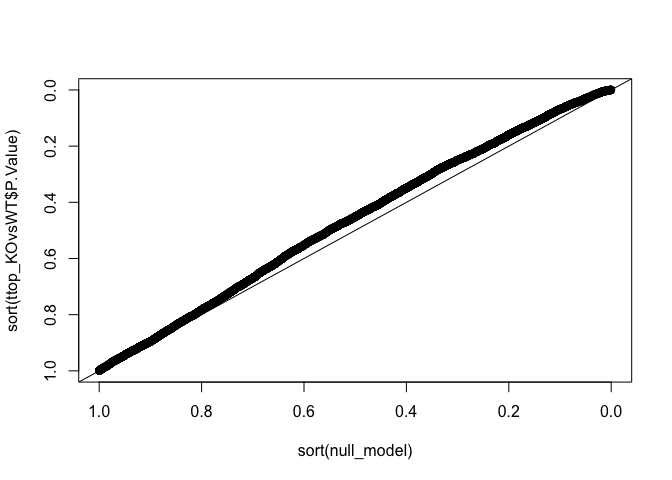
\includegraphics{02_differential_analysis_files/figure-latex/unnamed-chunk-3-1.pdf}

The qqplot (observed p-value distriubtion plotted against a random
baseline) is meant to give usan idea of the signal strength when
comparing KO and WT. The more the black dot line deviates from the
diagonal toward the upper part of the plot, the stronger the signal is.
This plot is very similar to a p-value histogram.

In this case, we can oberse a decent signal, but there are many context
where it could be much stronger. This type of difference is typical for
single mutations comapred to a wild type, which usually lead to weak
overall differences. Stronger differences are usually expected for
treatment vs control experiments, or when comparing tumor vs healthy
tissues.

\hypertarget{write-the-da-output}{%
\subsubsection{Write the DA output}\label{write-the-da-output}}

\begin{Shaded}
\begin{Highlighting}[]
\KeywordTok{write_csv}\NormalTok{(ttop_KOvsWT, }\StringTok{"results/ttop_KOvsWT.csv"}\NormalTok{)}
\end{Highlighting}
\end{Shaded}

\hypertarget{session-info-details}{%
\subsection{Session Info Details}\label{session-info-details}}

\begin{verbatim}
## R version 3.5.2 (2018-12-20)
## Platform: x86_64-apple-darwin15.6.0 (64-bit)
## Running under: macOS Mojave 10.14.6
## 
## Matrix products: default
## BLAS: /Library/Frameworks/R.framework/Versions/3.5/Resources/lib/libRblas.0.dylib
## LAPACK: /Library/Frameworks/R.framework/Versions/3.5/Resources/lib/libRlapack.dylib
## 
## locale:
## [1] en_US.UTF-8/en_US.UTF-8/en_US.UTF-8/C/en_US.UTF-8/en_US.UTF-8
## 
## attached base packages:
## [1] grid      stats     graphics  grDevices utils     datasets  methods  
## [8] base     
## 
## other attached packages:
## [1] hexbin_1.27.3   ggrepel_0.8.1   cowplot_1.0.0   gridExtra_2.3  
## [5] pheatmap_1.0.12 reshape_0.8.8   ggplot2_3.3.0   limma_3.38.3   
## [9] readr_1.3.1    
## 
## loaded via a namespace (and not attached):
##  [1] Rcpp_1.0.4         RColorBrewer_1.1-2 pillar_1.4.3      
##  [4] compiler_3.5.2     plyr_1.8.4         tools_3.5.2       
##  [7] digest_0.6.25      lattice_0.20-38    evaluate_0.14     
## [10] lifecycle_0.2.0    tibble_3.0.0       gtable_0.3.0      
## [13] pkgconfig_2.0.3    rlang_0.4.5        cli_2.0.2         
## [16] yaml_2.2.0         xfun_0.8           withr_2.1.2       
## [19] stringr_1.4.0      dplyr_0.8.5        knitr_1.23        
## [22] vctrs_0.2.4        hms_0.5.3          tidyselect_1.0.0  
## [25] glue_1.4.0         R6_2.4.1           fansi_0.4.1       
## [28] rmarkdown_1.14     purrr_0.3.3        magrittr_1.5      
## [31] scales_1.1.0       ellipsis_0.3.0     htmltools_0.3.6   
## [34] assertthat_0.2.1   colorspace_1.4-1   stringi_1.4.6     
## [37] munsell_0.5.0      crayon_1.3.4
\end{verbatim}


\end{document}
